
\subsubsection{電波フィンガープリントを用いた初期進行方向の補正}
% TODO:2. FPなのかフィンガープリントなのか統一した方がいいかも
% TODO: 無線基地局という表現結構よさげなので他での適用できると嬉しいかも
無線基地局の電波強度を用いた補正は効果的な手法であるが,基地局の正確な位置情報の取得が困難な場合がある.この課題に対する解決策として,電波強度の分布パターン(フィンガープリント)を利用した補正手法を実装している.この機能は前節で説明したWirelessSignalCorrectorクラスの一機能として提供している.

WirelessSignalCorrectorクラスの利用例をListing\ref{lst:rotate-trajectory-using-ble-fingerprint}に示す.
このクラスを利用するために必要な情報は2つある.1つ目は前節と同様の
歩行者が移動中に収集した信号スキャンデータである.2つ目は
フィンガープリントデータである.これは事前に環境内の様々な位置で
計測された各送信機のID,電波強度,およびその計測位置の座標が
記録されたデータベースである.前節とは異なり,この手法では基地局の
正確な位置情報は必要としない.

% TODO:3 WiressSignalCorrectorが被ってるのでキャプション名を変更した方がいいかも
\begin{lstlisting}[caption={WirelessSignalCorrectorの使用例},label=lst:rotate-trajectory-using-fingerprint,float=ht]
# フィンガープリントデータ
signal_fingerprints = pd.read_csv('fingerprints.csv')
# ts: 1234567890.123  # 計測時刻(秒)
# x: 15.2            # 計測位置のx座標(メートル)
# y: 24.8            # 計測位置のy座標(メートル)
# transmitter_id: "f2:65:d1:87:a4:2c"  # 送信機ID
# rssi: -68          # 電波強度(dBm)
# floor: "floor_5"   # フロア名

# WirelessSignalCorrectorの初期化と補正の実行
corrector = WirelessSignalCorrector(
    signal_realtime_scans=signal_realtime_scans,
    signal_fingerprints=signal_fingerprints,
    signal_threshold=-70
)
\end{lstlisting}

% TODO: 要修正:ここちょっと何言ってるのかわからない 
WirelessSignalCorrectorのFPを用いた補正処理は,歩行者から受信した各無線信号について,
受信時刻$t$ごとに位置推定を行う.
各時刻において,受信した送信機IDと同じデータポイントをFPデータベースから抽出する.
各データポイントの重み$w$は,受信時刻$t$におけるRSSI値$r_t$と,
FPデータベース内の同じビーコンのRSSI値$r_f$との差に基づいて,式\eqref{eq:weight}で計算される.
ここで,$\sigma$は電波強度の標準偏差を表すパラメータであり,
環境に応じて調整可能である.この式はガウシアンカーネルに基づいており,
RSSI値の差が小さいほど大きな重みが与えられる.

次に,これらの重みを用いて時刻$t$における推定位置$(p_x^t, p_y^t)$を式\eqref{eq:position}で計算する.
ここで,$(x_i, y_i)$はFPデータベース内の各データポイントの座標を表し,$
N_t$は時刻$t$において抽出されたデータポイントの総数である.
この重み付き平均により,その時刻のRSSI値と類似したデータポイントの座標がより強く反映された推定位置が得られる.
最適な回転角度の決定には,3.2.4節で導入した距離の総和$D(\theta)$を用いる.
ここでは,固定点として式\eqref{eq:position}で推定された位置$(p_x^t, p_y^t)$を使用する.
最適な回転角度$\theta_{\mathrm{opt}}$は,前節と同様に距離の総和を最小化する角度として決定される.
この手法の特徴は,基地局の正確な位置情報を必要としない点である.
その代わりに,事前に環境内で十分なFPデータを収集する必要がある.
ただし,環境の物理的な変化や人の往来,電波干渉などの要因により,FPデータは時間とともに劣化する可能性がある.
そのため,定期的なFPデータの更新が必要である.

\begin{equation}
\label{eq:weight}
w_t = \exp\left(-\frac{(r_t - r_f)^2}{2\sigma^2}\right)
\end{equation}

\begin{equation}
\label{eq:position}
p_x^t = \frac{\sum_{i=1}^{N_t} w_{t,i} x_i}{\sum_{i=1}^{N_t} w_{t,i}}, \quad
p_y^t = \frac{\sum_{i=1}^{N_t} w_{t,i} y_i}{\sum_{i=1}^{N_t} w_{t,i}}
\end{equation}

% TODO:2.パスロスモデルの比重も増やせる説明をした方がいいかも
% TODO:2.5 位置を推定した座標の図が欲しい
% TODO:2. 全体像を捉えて方向補正をするのが目的.なのでなんとなくこの辺にいそうというのが重要.
% 正確な位置を推定する必要はないといった方がいいかも
% TODO:2. 軌跡全体をみて最適化する形式だから十分なFPデータがなくても成り立つみたいな文が欲しい

% \begin{figure}[H]
%     \centering
%     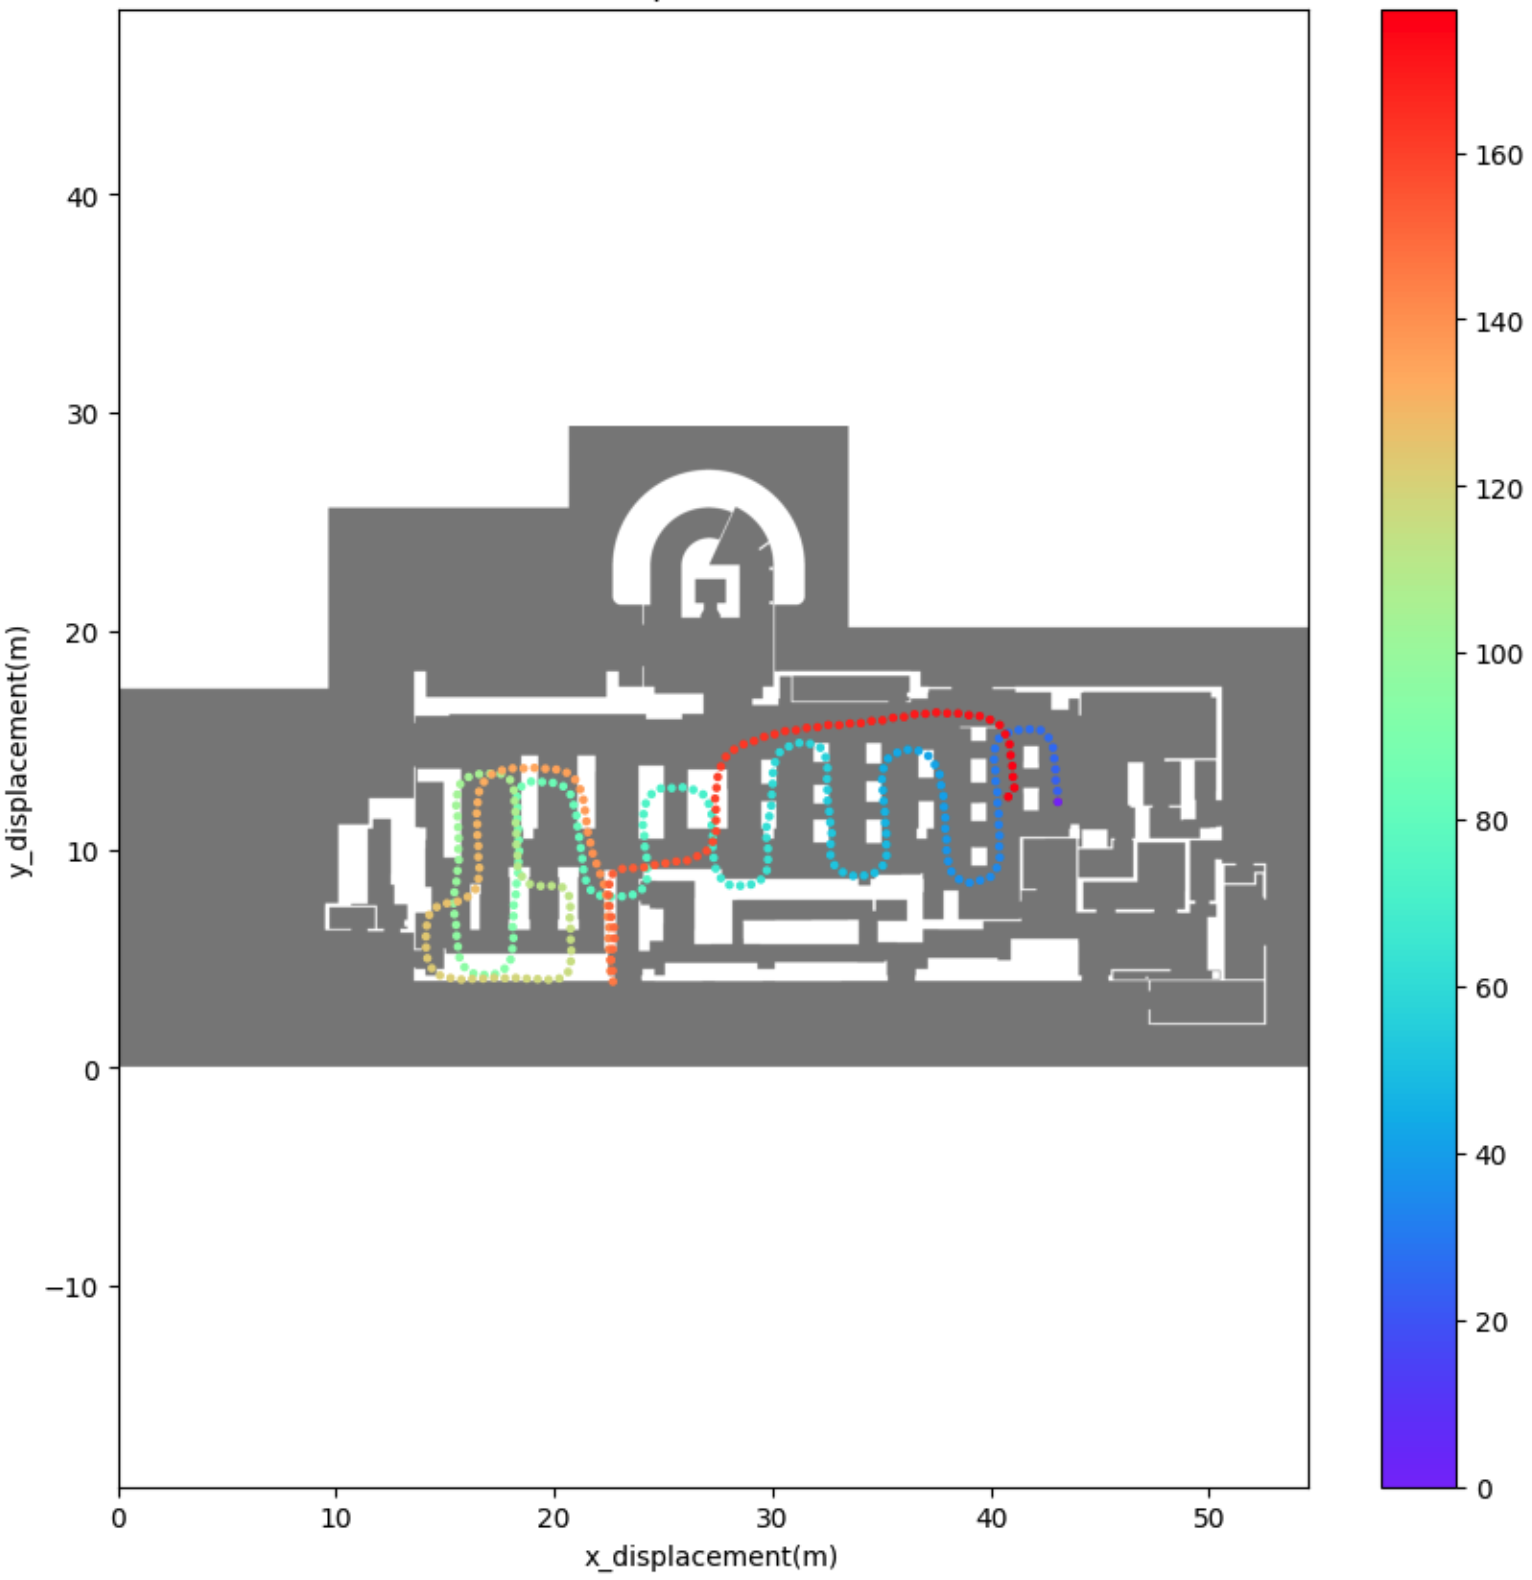
\includegraphics[width=\linewidth]{../image/fingerprint-rotate.jpg}
%     \caption{BLEのFPを用いた補正後の軌跡}    \label{fig:fingerprint-rotate}
% \end{figure}










